\section{Implementacja}
\subsection{Narzędzia}
W celu ułatwienia pracy kilku osób nad projektem zostało wykorzystane narzędzie GitHub \cite{github}. Zastosowano również ciągłą integrację wykorzystując Travis CI \cite{travis}. Do automatyzuji budowy oprogramowania na platformę Java użyto Apache Maven \cite{maven}.

\subsection{Środowisko}
Do stworzenia klienta aplikacji użyto środowiska Visual Studio Code. Część serwerowa powstała w~środowisku Eclipse EE z~wykorzystaniem
serwera aplikacyjnego WildFly \cite{wildFly_doc} oraz bazy danych MySQL. Tabele bazy danych zostaną utworzone
przy pierwszym uruchomieniu serwera. Należy skonfigurować serwer WildFly tak, aby mógł korzystać z~baz danych MySQL. 

\subsection{Serwer}
Do zadań serwera należy zarządzanie przechowywanymi informacjami oraz ich
udostępnianie. Został on stworzony w~technologii Java EE. Kod podzielono na warstwy: danych (model), logiki (managery), oraz interfejs wejściowy (REST). Warstwa danych odpowiada za przechowywanie informacji w~bazie danych oraz dostęp do nich. Warstwa logiki realizuje funkcje takie jak np. wgrywanie zdjęcia, czy rejestracja użytkownika. Interfejs REST przyjmuje żądania HTTP, wyodrębnia z~nich dane i~przekazuje je do warstwy logiki. Generując odpowiedź tworzy on odpowiedź HTTP, ustalając dla niej m.in. odpowiedni kod odpowiedzi oraz treść.

\subsubsection{Model}
W celu stworzenia bazy danych przedstawionej w~projekcie aplikacji utworzono
klasy modelowe. Są to zwykłe klasy Javy opatrzone specjalnymi adnotacjami.
Umieszczone one zostały w~pakiecie photoGallery.model. Przykład takiej klasy
przedstawiono na listingu \ref{lst:image}. Za pomocą adnotacji są w
niej tworzone klucze główne (adnotacja @Id oraz @GeneratedValue do
automatycznego generowania wartości) oraz klucze obce (adnotacje @ManytoOne oraz
@JoinColumn). Dodatkowo definiowane są także zapytania,
które będą mogły być później
wykorzystane (@NamedQuery). 

\lstinputlisting[caption={Fragment klasy modelu Image, pominięto metody oraz pola nie posiadające adnotacji}, label=lst:image]
{listings/Image.java}

Do wykonywania operacji na bazie danych wykorzystano klasy DAO. Każda klasa
modelu posiada swoją własną klasę DAO. Klasy te można znaleźć w~pakiecie
photoGallery.dao. Ze względu na to, że wszystkie posiadają podobne funkcje
stworzono abstrakcyjną klasę generyczną GenericDAO. Dostarcza ona podstawowych
operacji takich jak wyszukanie w~bazie obiektu po identyfikatorze, jego
tworzenie, modyfikacja oraz usuwanie, a także pobieranie wszystkich obiektów. Klasa ta została przedstawiona na listingu
\ref{lst:genericDAO}. DAO konkretnej klasy rozszerza generyczne DAO oraz, jeśli
to potrzebne, dodaje dodatkowe metody. Przykład klasy DAO pokazano na listingu \ref{lst:UserDAO}. Rozszerza ona klasę GenericDAO podając typ danych na jakich będzie operowała oraz implementuje metodę GetClassType().

\newpage
\lstinputlisting[caption={Klasa GenericDAO}, label=lst:genericDAO]
{listings/GenericDAO.java}

\lstinputlisting[caption={Klasa UserDAO}, label=lst:UserDAO]
{listings/UserDAO.java}

\subsubsection{\textcolor{red}{Logika aplikacji}}
Logika aplikacji, realizująca jej funkcjonalności po stronie serwera, została umieszczona w~klasach Managerów (znajdującą się one w~pakiecie photoGallery.manager). Są to bezstanowe komponenty sesyjne EJB. Każda ich metoda realizuje jedno polecenie, które jest niezależne od innych. Managery posiadają dostęp do DAO dzięki wstrzykiwaniu zależności (ang. dependency injection). Na listingu
\ref{lst:UserManager} przedstawiono klasę UserManager, która zajmuje się
operacjami na użytkownikach - procesem rejestracji i logowania. Adnotacja w~wierszu pierwszym informuje o~tym, że klasa ta
jest bezstanowym EJB. Wiersze 4-5 odpowiadają za wstrzyknięcie DAO
odpowiedzialnego za operacje na tabeli przechowującej dane użytkowników.
Metoda loginUser() (wiersze 9-21) przyjmuje jako parametry login oraz
hasło użytkownika. Po udanym logowaniu zwracany jest obiekt użytkownika, w
przeciwnym wypadku zgłaszany jest wyjątek logowania. Występuje on w~przypadku
gdy hasło jest niepoprawne, a także gdy nie istnieje użytkownik o~podanym loginie. Proces logowania przebiega następująco:
\begin{itemize}
	\item pobranie użytkownika o~podanym loginie, jeśli nie istnieje zgłoszenie wyjątku (wiersze 10-12),
        \item wygenerowanie hashu z~hasła (wiersz 13. oraz metoda generateHash() w~wierszach 27-42),
	\item porównanie wygenerowanego hashu z~zapisanym w~bazie oraz zgłoszenie wyjątku jeśli nie są identyczne (wiersze 13-16),
	\item wygenerowanie tokena i~zapisanie go w~bazie (wiersze 17-19 oraz metoda generateToken() w~wierszach 23-25),
	\item czyszczenie pola zwierającego hash hasła, modyfikacja ta dotyczy tylko obiektu zwracanego przez funkcje, nie ma wpływu na dane w~bazie danych (wiersz 19.).
\end{itemize}

\lstinputlisting[caption={Klasa UserManager}, label=lst:UserManager]
{listings/UserManager.java}

\subsubsection{\textcolor{red}{Interfejs wejściowy}}
Dostęp do logiki aplikacji został udostępniony poprzez interfejs REST stworzony
przy użyciu standardu JAX-RS. W celu kontroli dostępu do aplikacji
(ochrona przed niezalogowanymi użytkownikami) został utworzony filtr przechwytujący wchodzące zapytania (listing \ref{lst:filter}). 
Pobiera on zawartość nagłówka \textit{AUTHORIZATON}, a następnie, dzięki wstrzykniętemu managerowi użytkowników, decyduje czy żądanie może zostać przepuszczone dalej. W nagłówku znajduje się login użytkownika oraz token wygenerowany w~trakcie procesu logowania. W przypadku, gdy token będzie niepoprawny, żądanie zostanie przerwane z~kodem odpowiedzi \textit{UNAUTHORIZED}.

\lstinputlisting[caption={Klasa LoginFilter}, label=lst:filter]
{listings/LoginFilter.java}

Nie każda metoda jest chroniona przed dostępem niezalogowanych użytkowników. Metody chronione są oznaczone adnotacją, którą jest też oznaczony filtr (adnotacja @Secured przedstawiona na listingu \ref{lst:securedAnnotation}).

\lstinputlisting[caption={Adnotacja @Secured}, label=lst:securedAnnotation]
{listings/Secured.java}

Na listingu \ref{lst:ImageRestEndpoint} został przedstawiony fragment klasy będącej punktem wejścia do serwera odpowiedzialnym za zdjęcia. Za pomocą adnotacji oznaczono ścieżkę oraz typ danych, które przyjmują oraz zwracają metody danej klasy. Dodatkowo każda metoda jest opatrzona adnotacją z~konkretną ścieżką oraz z~metodą HTTP jaką obsługuje. Każda metoda zwraca obiekt typu Response, który reprezentuje odpowiedź HTTP. Poprzez ten obiekt ustawiany jest kod odpowiedzi oraz jej treść w~formacie JSON.

\lstinputlisting[caption={Fragment klasy ImageRestEndpoint}, label=lst:ImageRestEndpoint]
{listings/ImageRestEndpoint.java}

\subsection {Klient}
Aplikacja kliencka została wykonana w framework'u Angular 5, co wiązało się z podzieleniem jej na kilka komponentów, które pełniły odpowiednią role w systemie. Utworzone więc następujące komponenty:
\begin{itemize}
	\item welcome-page-component (strona główna) - odpowiedzialny za wyświetlanie strony głownej, 
	\item login-page-component (logowanie) - odpowiada za logowanie użytkownika,
	\item register-page (rejestracja) - służy do rejestracji 
	\item add-image-page (dodawanie nowego obrazu) - za pomocą tego komponentu zalogowany użytkownik może dodać nowy obraz do systemu,
	\item get-photo-page (wyszukiwanie obrazów) - udostępnia wyszukiwarkę, dzięki której użytkownik może za pomocą odpowiednich filtrów wyświetlić odpowiednie zdjęcie.a
	
\end{itemize}

\subsubsection{Interfejs graficzny}
Interfejs graficzny stworzono wykorzystując biblitekę Angular Material . Po
uruchomieniu aplikacji, ukaże się strona główna serwisu (rysunek \ref{fig:welcome}). Za pomocą przycisków, które są umieszczone po prawej stronie headera użytkownik może się zalogwać (rysunek \ref{fig:login}) lub zarejestrować (rysunek \ref{fig:register}). Po zalogowaniu otwierają się możliwości przejścia do panelu dodawania nowego zdjęcia (rysunek \ref{fig:newPhoto}) oraz przeglądania już istniejących (rysunek \ref{fig:searchPhoto}).
\begin{figure}
	\centering
	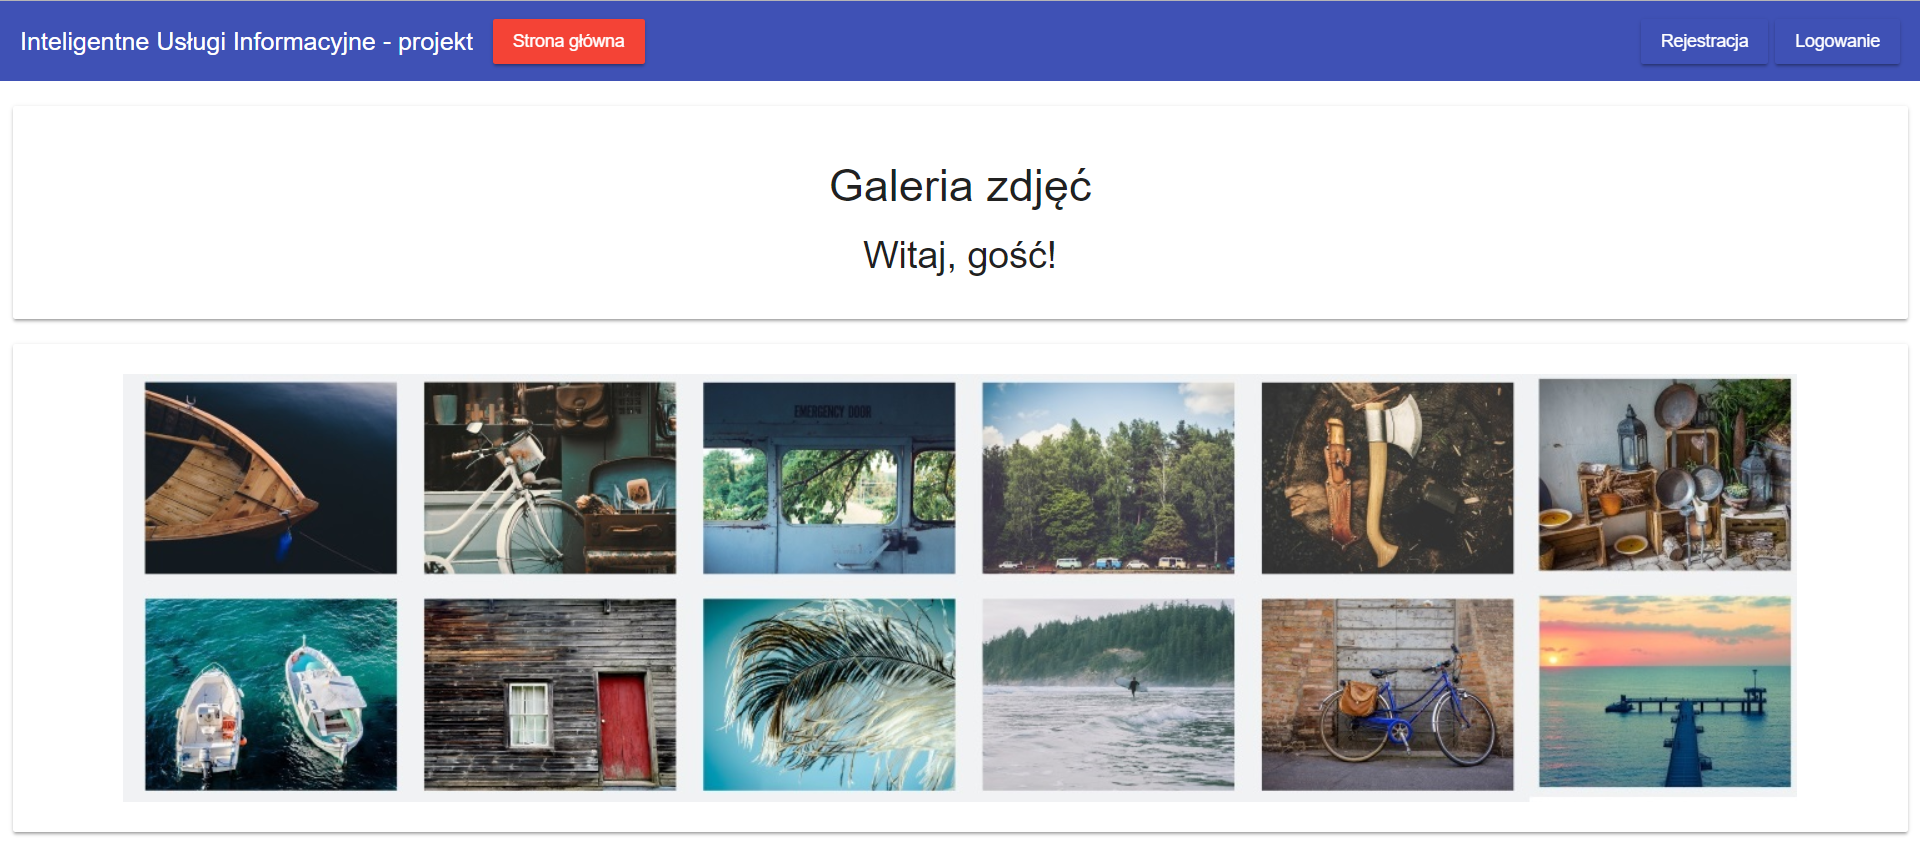
\includegraphics[width = 15cm]{images/e_g.png}
	\caption{Strona główna serwisu
		\newline Źródło: opracowanie własne}
	\label{fig:welcome}
\end{figure}
\begin{figure}
	\centering
	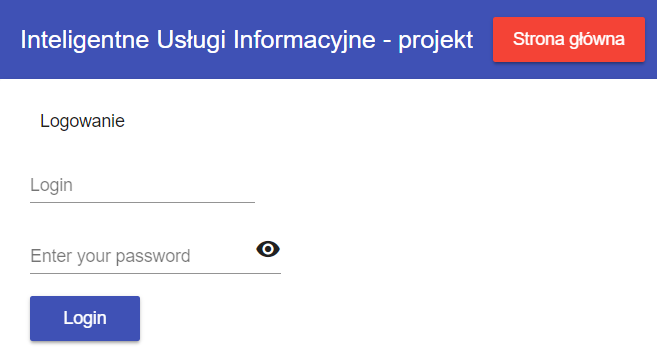
\includegraphics[width = 15cm]{images/logowanie.png}
	\caption{Logowanie
		\newline Źródło: opracowanie własne}
	\label{fig:login}
\end{figure}
\begin{figure}
	\centering
	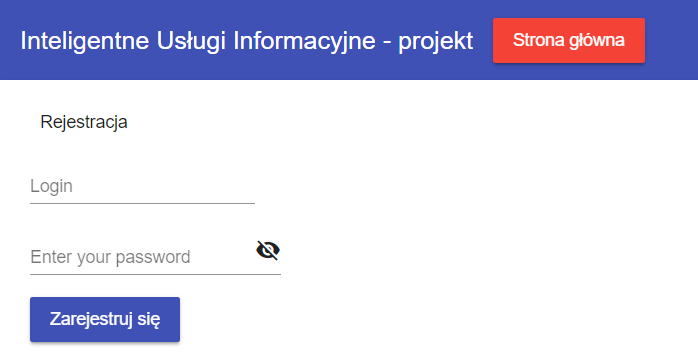
\includegraphics[width = 10cm]{images/rejestracja.png}
	\caption{Rejestracja
		\newline Źródło: opracowanie własne}
	\label{fig:register}
\end{figure}
\begin{figure}
	\centering
	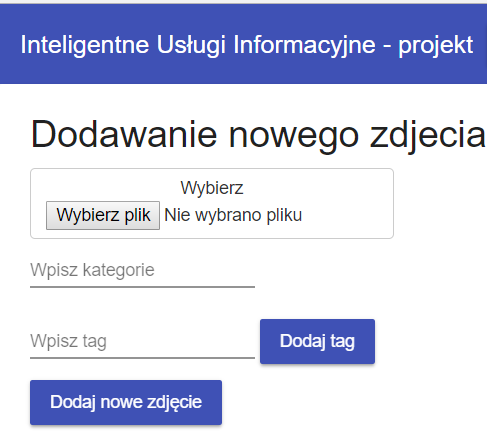
\includegraphics[width = 10cm]{images/nowe_zdjecie.png}
	\caption{Dodawanie nowego zdjęcia
		\newline Źródło: opracowanie własne}
	\label{fig:newPhoto}
\end{figure}
\begin{figure}
	\centering
	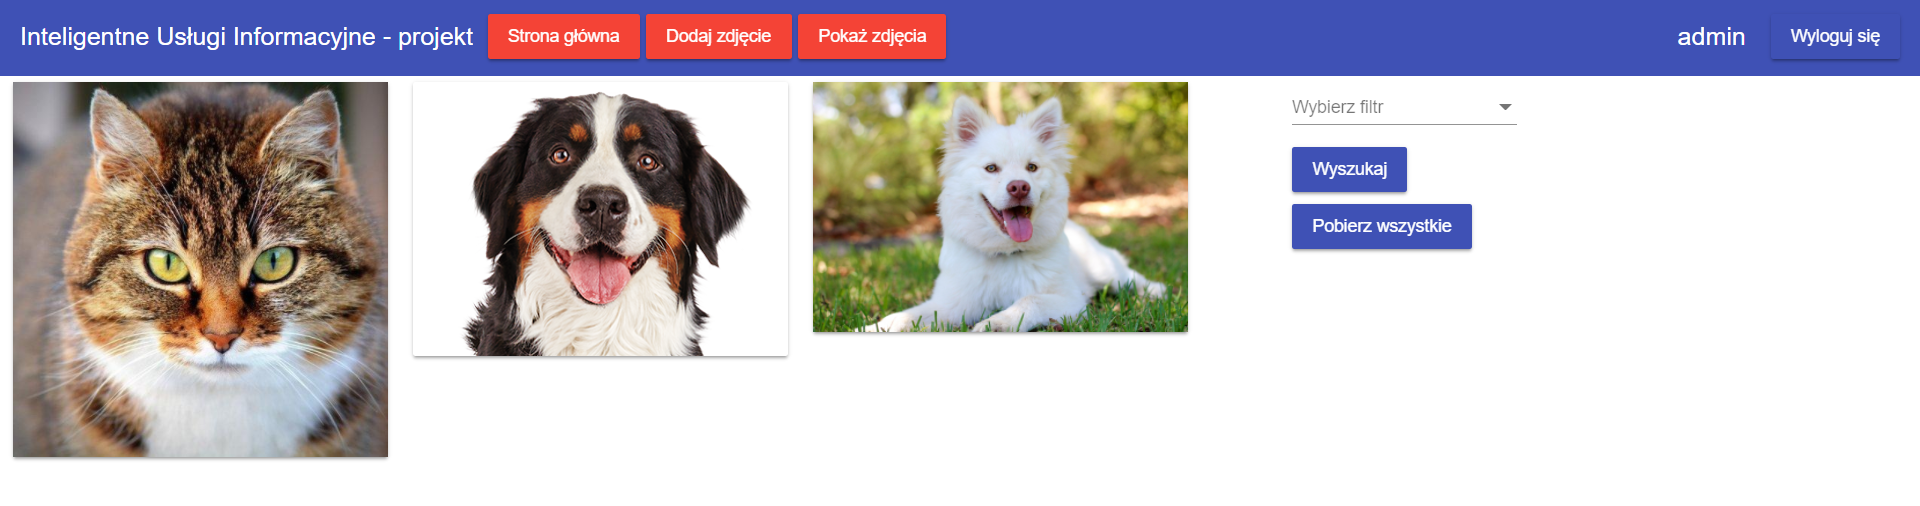
\includegraphics[width = 15cm]{images/search.png}
	\caption{Wyszukiwanie zdjęć 
		\newline Źródło: opracowanie własne}
	\label{fig:searchPhoto}
\end{figure}



